%\documentclass[12pt,twocolumn]{article}
\documentclass[12pt]{article}
\usepackage{amsmath,amssymb,bm}
\usepackage{graphicx}
\usepackage[hidelinks]{hyperref}
\usepackage[margin=1.2in]{geometry}
\usepackage{float}
\usepackage{wrapfig}
\usepackage{bigints}
\usepackage{physics}
\usepackage{xcolor}
\hypersetup{
	colorlinks,
	linkcolor={red!50!black},
	citecolor={blue!50!black},
	urlcolor={blue!80!black}
}

\title{Graduate school project report\\
	Halo formation in the cosmic web}

\author{ PremVijay V \qquad Supervisor: Prof. Aseem Paranjape}


\begin{document}

\maketitle

\hyphenpenalty=5000

\begin{abstract}
abstract
\end{abstract}

\section{Introduction}
Cosmic Microwave Background (CMB) shows that the Universe was initially homogenous with very small inhomogeneities. Thanks to the attractive gravitational force, those inhomogeneities led to the formation of galaxies. And the universe we see today has a lot of interesting structures well beyond the galactic scale. This foam-like \ref{fig:orangepie} large scale structure of the universe is called the cosmic web. 

\begin{wrapfigure}[17]{r}{0.6\linewidth}
\centering
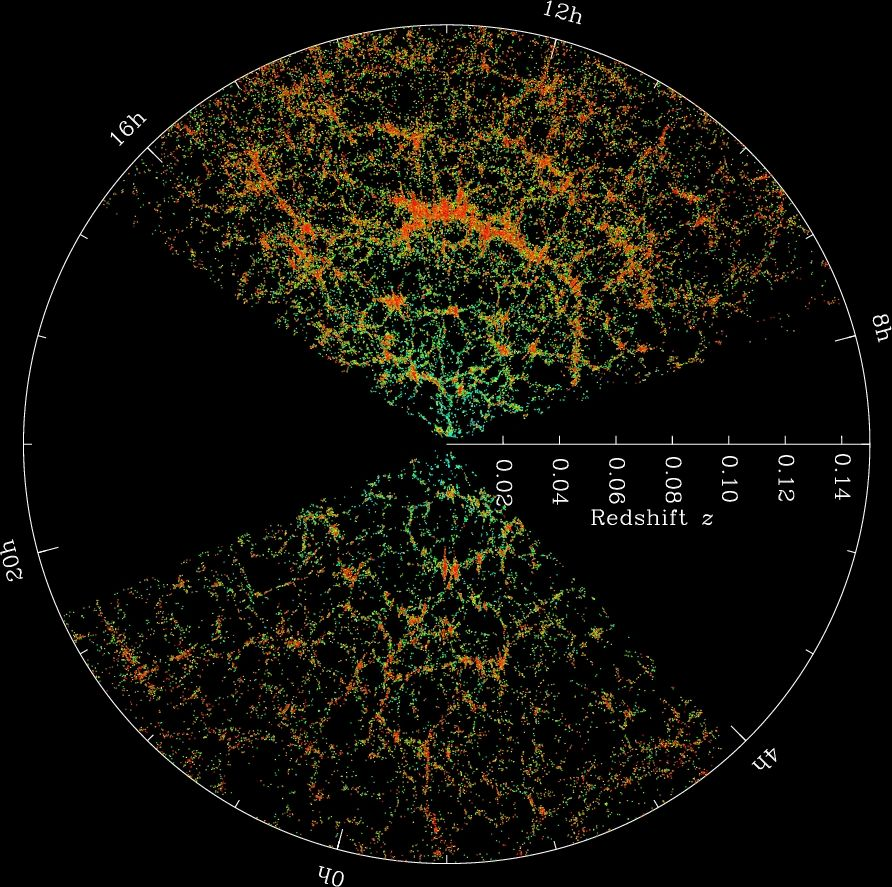
\includegraphics[width=0.9\linewidth]{orangepie}
\caption{ \textit{Large Scale Structure revealed by \cite{cite_sdss}}}
\label{fig:orangepie}
\end{wrapfigure}

%\begin{figure}[tbh]
%	\centering
%	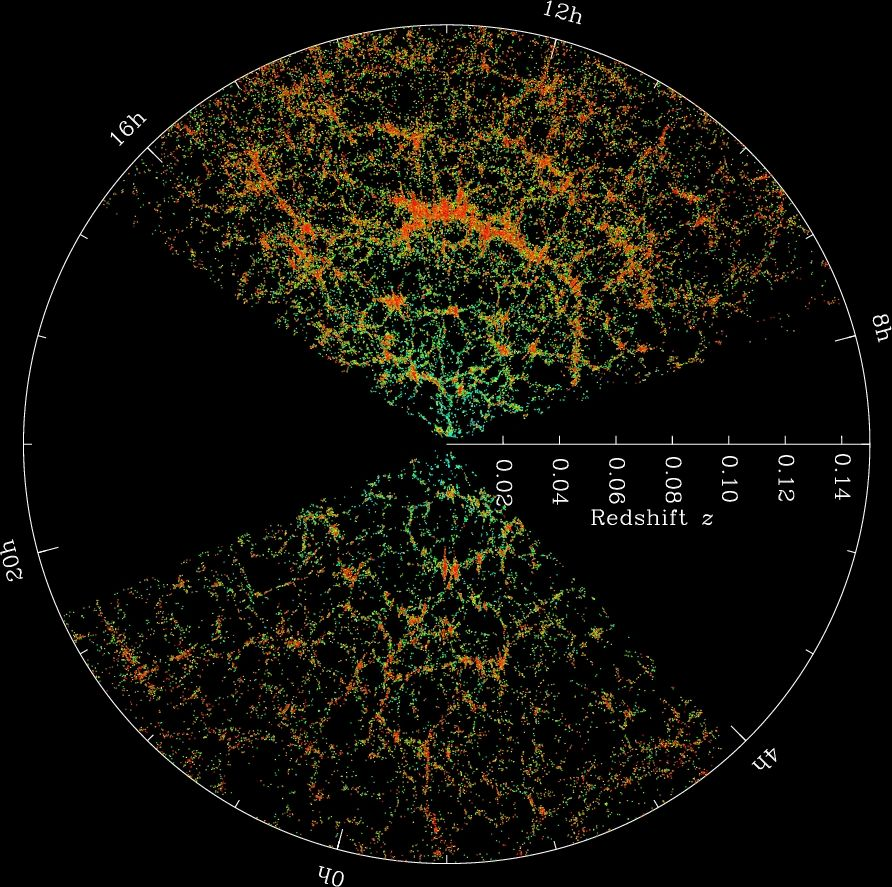
\includegraphics[width=0.9\linewidth]{orangepie}
%	\caption{ Large Scale Structure (LSS) revealed by \cite{cite_sdss}}
%	\label{fig:orangepie}
%\end{figure}
%\noindent
Understanding the statistical properties of the large scale structure and its evolution is crucial to test and constrain cosmological models. Computer simulations can be used to evolve initial inhomogeneities to the structure we see today and hence can be compared with sky survey observations.


\section{Analytical tools}
Though the evolution of large scale structure can be simulated, we need analytical tools to get a deeper understanding and also to make generic constraints that can be tested by observations. On the other hand, simulations help in making and refining these analytical tools. 

\subsection{FLRW background}
We assume the standard $\Lambda$CMD model without any curvature. The FLRW metric for the homogeneous background in comoving coordinates is
\begin{align}
ds^2 &= -dt^2 + a^2(t) d\vec{x}^2\\
&= a^2(\tau) \left( -d\tau^2 + d\vec{x}^2 \right) 
\end{align}
where $\tau$ is defined as the conformal time.\\
Let $\bar{\rho}_{m}$ and $\bar{\rho}_{\Lambda}$ denote the mean matter density and mean dark energy density. Hubble parameter is defined as $H \equiv \dot{a}/a$ where the dot denotes derivative with respect to time '$t$'. At the zeroth order, the Einstein equations reduces to the Friedmann equations,
\begin{align}
%H^2 = \frac{8 \pi G}{3} \bar{\rho} = \frac{8 \pi G}{3} \left( \bar{\rho}_{m} + \bar{\rho}_{\Lambda} \right) \\ 
\nonumber
H^2 = \left(\frac{\dot{a}}{a}\right)^2 &= \frac{8 \pi G}{3} \bar{\rho} \\
\label{eq:fried-eqn-1}
&= \frac{8 \pi G}{3} \left( \bar{\rho}_{m} + \bar{\rho}_{\Lambda} \right) \\
\nonumber
\dot{H} + H^2 = \frac{\ddot{a}}{a} &= - \frac{4\pi G}{3} \left(\bar{\rho} + 3\bar{p} \right)\\
\nonumber
&= - \frac{4\pi G}{3} \left[ \bar{\rho}_{m} + \bar{\rho}_{\Lambda} + 3 (0 -\bar{\rho}_{\Lambda}) \right]\\
\label{eq:fried-eqn-2}
&= - \frac{4\pi G}{3} \left[ \bar{\rho}_{m} - 2 \bar{\rho}_{\Lambda} \right] 
%\label{eq:fried-eqn-2}
\end{align}
%
Assuming that the matter and dark energy are independently conserved,
\begin{align}
\dot{\bar{\rho}}_{m} &= -3 H \left(\bar{\rho}_{m} + {\bar{p}_{m}}\right) = - 3 H \bar{\rho}_{m} \\
\dot{\bar{\rho}}_{\Lambda} &= -3 H \left(\bar{\rho}_{\Lambda} + \bar{p}_{\Lambda} \right) = 0
\end{align}
Solving the above equations give $\bar{\rho}_{m} \propto a^{-3}$ and $\bar{\rho}_{\Lambda}$ is constant.\\
Density parameters are defined as
\begin{align}
\Omega_{m} \equiv \frac{8 \pi G \bar{\rho}_{m}}{3 H^2} \quad
\Omega_{\Lambda} \equiv \frac{8 \pi G \bar{\rho}_{\Lambda}}{3 H^2}
\end{align}
%
so that the first Friedmann equation \ref{eq:fried-eqn-1} reduces to $\Omega_{m} + \Omega_{\Lambda} = 1$. Let us now switch to conformal time '$\tau$' and define conformal Hubble parameter $\mathcal{H} \equiv \partial_\tau a / a = \dot{a}$.
\begin{align}
3 H^2 \Omega_{m} &= 8 \pi G \bar{\rho}_{m}\\
3 \mathcal{H}^2 \Omega_{m} &= 8 \pi G \bar{\rho}_{m} a^2 \label{eq:omega-m-relation}
\end{align}
The second Friedmann equation \eqref{eq:fried-eqn-2} becomes 
\begin{align}
- \frac{4\pi G}{3} \left[ \bar{\rho}_{m} - 2 \bar{\rho}_{\Lambda} \right] &=  \frac{\ddot{a}}{a} = \frac{\dot{\mathcal{H}}}{a}\\
- \frac{4\pi G}{3} \left[ \bar{\rho}_{m} - 2 \bar{\rho}_{\Lambda} \right] a^2 &= \frac{d \mathcal{H}}{a^2 d\tau} a^2\\
\label{eq:fried-eqn-2-simple}
\mathcal{H}^2 \left[ - \frac{\Omega_{m}}{2} + \Omega_{\Lambda} \right] &= \frac{d \mathcal{H}}{d\tau}\\
\Omega_{\Lambda} - \frac{\Omega_{m}}{2} &= \frac{d \mathcal{H}}{d\tau} \mathcal{H}^{-2} = \frac{d \mathcal{H}}{\mathcal{H} d\tau} \mathcal{H}^{-1}\\
&= \frac{d \ln \mathcal{H}}{d\tau}
\left[ \frac{da}{a d\tau} \right]^{-1} = \frac{d \ln \mathcal{H}}{d \ln a}
\end{align} 
It is useful to define another time evolution parameter $y \equiv \ln a$.
%so that the equation \eqref{eq:fried-eqn-2-simple} becomes
\begin{align}
\Omega_{\Lambda} - \frac{\Omega_{m}}{2} &= \frac{d \ln \mathcal{H}}{d y} 
\end{align}

\subsection{Growth of Structure}
While the evolution of background cosmology can be studied fully analytically, the inhomogeneities responsible for structure formation can't be solved exactly without making any ansatz. We will look into different approaches but first let us setup the equations. Since a large fraction of the matter in the Universe is dark matter, gravity plays the major role in structure formation. While we can directly apply the Einstein equations of general relativity, we take a simpler approach by starting with the Newtonian fluid equations.




\subsubsection{Newtonian equations in inhomogeneous $\Lambda$CDM Universe}
%Since dark matter only by gravity, we can start with 
%The density contrast and relative velocity Large scale structure is the density
%Let us define the quantities  
The matter density contrast can be quantified in terms of overdensity field $\delta$,
\begin{align}
%\nonumber
\delta (\vec{x}, \tau) &\equiv \frac{{\rho}_{m} (\vec{x}, \tau) -\bar{\rho}_{m} (\tau) }{\bar{\rho}_{m} (\tau)} \quad
= \frac{{\rho}_{m} (\vec{x}, \tau) }{\bar{\rho}_{m} (\tau)} - 1
\end{align}
The velocity field is then defined as
\begin{align}
\vec{v} (\vec{x}, \tau) &\equiv \frac{d \vec{r}}{dt} = \frac{d }{dt} (a \vec{x})\\
&= \frac{1}{a} \frac{d }{d \tau} (a \vec{x})\\
&= \frac{da/d \tau}{a} \vec{x} + \frac{d \vec{x}}{d \tau}\\
&= \mathcal{H} (\tau) ~\vec{x} + \vec{u} (\vec{x}, \tau)
\end{align}
where $\vec{u} (\vec{x}, \tau) \equiv d \vec{x} / d\tau$ is called the peculiar velocity, while the first term quantifies the Hubble flow. Due to the time dependance of $\mathcal{H}$, there is an associated acceleration purely due to hubble flow. That acceleration can be found by setting peculiar velocity to zero. 
\begin{align}
\frac{d}{dt} \left( \mathcal{H} (\tau) ~\vec{x} \right) &= \frac{d}{dt} \frac{da}{dt}  ~\vec{x}\\
&= \ddot{a}(t) ~\vec{x} = \frac{1}{a} \ddot{a}(t) ~\vec{r}
\end{align}
This acceleration can be written in terms of a potential
\begin{align}
\bar{\phi} \equiv - \frac{1}{2} a \ddot{a} ~\left| \vec{x}\right| ^2 &= - \frac{1}{2} \frac{\ddot{a}}{a} ~\left| \vec{r}\right| ^2\\
\implies \nabla_{r} \bar{\phi} &= \frac{\ddot{a}}{a} ~\vec{r}
\end{align}
Let $\phi$ denote the total gravitational potential in the presence of inhomeneities. We can define the modified gravitaional potential as $\Phi \equiv \phi - \bar{\phi}$.

Evolution of the density inhomogeneity $\delta$, the peculiar velocity field  $\vec{u}$, and the modified potential $\Phi$ is described by the continuity equation, Euler equation and Poisson equation.
\begin{align}
\partial_{\tau} \delta + \nabla \cdot \left[ (1+ \delta) \vec{u} \right] &= 0\\
\partial_{\tau} \vec{u} + \mathcal{H} \vec{u} + \left( \vec{u} \cdot \nabla \right)  \vec{u} &= - \nabla \Phi\\
\nabla^2 \Phi &= \frac{3}{2} \mathcal{H}^2 \Omega_{m}(\tau) \delta
\end{align}
where $\nabla$ is with respect to comoving coordinates.


\subsubsection{Linear solutions to inhomogeneous CDM}
If the inhomogeneities are small then we can consider them as perturbation to the homogeneous background. To the first order of perturbation, the equations are linear.
\begin{align}
\label{eq:cont-linear}
\partial_{\tau} \delta + \nabla \cdot \vec{u} &= 0\\
\label{eq:euler-linear}
\partial_{\tau} \vec{u} + \mathcal{H} \vec{u} &= - \nabla \Phi\\
\label{eq:poisson-linear}
\nabla^2 \Phi &= \frac{3}{2} \mathcal{H}^2 \Omega_{m}(\tau) \delta
\end{align}
Taking divergence of \eqref{eq:euler-linear}
\begin{align}
%\nonumber
\partial_{\tau} \nabla \cdot  \vec{u} + \mathcal{H} \nabla \cdot  \vec{u} &= - \nabla^2 \Phi \\
\intertext{substituting for $\nabla \cdot \vec{u}$ from \eqref{eq:cont-linear} and for $\nabla^2 \Phi$ from \eqref{eq:poisson-linear}}
\partial_{\tau} (-\partial_{\tau} \delta) + \mathcal{H} (-\partial_{\tau} \delta) &= - \frac{3}{2} \mathcal{H}^2 \Omega_{m}(\tau) \delta\\
\partial_{\tau}^2 \delta + \mathcal{H} \partial_{\tau} \delta &= \frac{3}{2} \mathcal{H}^2 \Omega_{m}(\tau) \delta \label{eq:delta-lin}
\end{align}
In the last equation, there is no spatial derivatives, so it is just a second order ordinary differential equation for $\delta$. In general, the solution is of the form,
\begin{align}
\delta (\vec{x}, \tau) &= A(\vec{x}) D_1^{(+)}(\tau) + B(\vec{x}) D_1^{(-)}(\tau) 
\end{align}
where $D_1^{(+)}(\tau)$ denotes growing mode and $D_1^{(-)}(\tau)$ denotes decaying mode. 
The divergence of peculiar velocity is then
\begin{align}
\theta  (\vec{x}, \tau) &\equiv \nabla \cdot  \vec{u} = -\partial_{\tau} \delta\\
&= - A(\vec{x}) \frac{d D_1^{(+)}}{d \tau} - B(\vec{x}) \frac{d D_1^{(-)}}{d \tau} 
\end{align}
The growing mode and decaying mode can be obtained by directly solving the linear ODE \eqref{eq:delta-lin}. Before going into the full solution, let us look into the matter dominated era where $\Omega_{m}(\tau) \approx 1$. 
Inserting this in the background equation \eqref{eq:omega-m-relation} we get,
\begin{align}
\mathcal{H} &\propto \sqrt{\bar{\rho}_{m} a^2} \propto a^{-1/2}\\
\implies \frac{da}{d\tau} &\propto a^{1/2} \implies
a^{-1/2} da \propto d \tau\\
\intertext{We can solve for scale factor evolution by integrating the above equation.}
a(\tau) &\propto \tau^2 \quad \implies \mathcal{H}(\tau) = \frac{2}{\tau}\\
H(\tau) &= \frac{\dot{a}}{a} = \frac{\mathcal{H}}{a} \propto \tau^{-3}
\end{align}
Hence the linear perturbation equation \eqref{eq:delta-lin} reduces to,
\begin{align}
\partial_{\tau}^2 \delta + \mathcal{H} \partial_{\tau} \delta &= \frac{3}{2} \mathcal{H}^2 \delta\\
\partial_{\tau}^2 \delta + \frac{2}{\tau} \partial_{\tau} \delta &= \frac{3}{2} \left( \frac{2}{\tau} \right) ^2 \delta\\
\partial_{\tau}^2 \delta + \frac{2}{\tau} \partial_{\tau} \delta &- \frac{6}{\tau^2} \delta = 0
\end{align}
By assuming power law solution, we get the growing mode $D_1^{(+)}(\tau) \propto \tau^2 \propto a(\tau)$ and the decaying mode $D_1^{(-)}(\tau) \propto \tau^{-3} \propto  H(\tau)$.\\
It turns out that even after dark energy starts to dominate, the decaying mode stays proportional to the Hubble parameter $D_1^{(-)}(\tau) \propto H(\tau)$. However, now the time dependence of Hubble parameter $H(\tau)$ is different.  \\
Similarly, the growing mode can be generalised to an integral involving $H(\tau)$,
\begin{align}
D_1^{(+)}(\tau) &\propto H(\tau) \int^{\tau} \frac{1}{a(\tau') H^2(\tau')} d\tau'\\
\implies D_1^{(+)}(a) &\propto H(a) \int^{a} \frac{1}{(a'H(a'))^3} da'
\end{align}
We can set the proportionality constant by setting $D_1^{(+)}(a) = a$ during matter dominated phase.
\begin{align}
D_1^{(+)}(a) &= \frac{5}{2} \Omega_{m0} \frac{H(a)}{H_0} \int^{a} \frac{1}{(a'H(a')/H_0)^3} da'
\end{align}

\subsubsection{Eulerian perturbation theory}
We will switch to Fourier space with respect to spatial comoving coordinates. The density inhomogeneity parameter in the Fourier space is defined as
\begin{align}
\delta_{\vec{k}}(\tau) \equiv \int d^3k ~e^{-i \vec{k} \cdot \vec{x}} ~\delta(\vec{x},\tau), \qquad
\delta (\vec{x},\tau) &= \int \frac{d^3k}{(2\pi)^3} ~e^{i \vec{k} \cdot \vec{x}} ~\delta_{\vec{k}}(\tau)
\end{align}
Similarly we can define Fourier space variables $\theta_{\vec{k}}(\tau), ~\vec{u}_{\vec{k}}(\tau) ~\&~ \Phi_{\vec{k}}(\tau)$ corresponding to $\theta (\vec{x},\tau), \vec{u} (\vec{x},\tau) ~\&~ \Phi (\vec{x},\tau)$.

The linear partial differential equations \eqref{eq:cont-linear}, \eqref{eq:euler-linear} \& \eqref{eq:poisson-linear} become linear ordinary differential equations in Fourier space and hence each wavemode evolves independently.
\begin{align}
\partial_{\tau} \delta_{\vec{k}} + \theta_{\vec{k}} &= 0\\
\partial_{\tau} \theta_{\vec{k}} + \mathcal{H} \theta_{\vec{k}} - k^2 ~\Phi_{\vec{k}} &= 0\\
-k^2 ~\Phi_{\vec{k}} &= \frac{3}{2} \mathcal{H}^2 \Omega_{m}(\tau) ~\delta_{\vec{k}}
\end{align}
However when we include non-linear terms, Fourier wavemodes are coupled. Let us assume that there is no vorticity, $\nabla \times \vec{u} = 0$ so that the divergence-less term is zero.  Fourier transforming the continuity equation, we get

\begin{align}
\label{eq:cont-eqn-fourier}
\partial_{\tau} \delta_{\vec{k}} + \theta_{\vec{k}} &= - \bigint \frac{d^3k_1 d^3k_2} { (2 \pi)^3} ~\frac{\vec{k}_1 \cdot \left( \vec{k}_1 + \vec{k}_2 \right) }{k_1^2}  ~\delta_{\vec{k}_2} ~\theta_{\vec{k}_1} ~\delta_D \left( \vec{k} - \left[ \vec{k}_1 + \vec{k}_2 \right] \right)
\end{align}
Fourier transforming the divergence of Euler equation, we get
\begin{align}
\label{eq:euler-eqn-fourier}
\partial_{\tau} \theta_{\vec{k}} + \mathcal{H} \theta_{\vec{k}} - k^2 ~\Phi_{\vec{k}} &= - \bigint \frac{d^3k_1 d^3k_2} { (2 \pi)^3} ~\frac{\left( \vec{k}_1 \cdot \vec{k}_2 \right) \left| \vec{k}_1 + \vec{k}_2 \right|^2 }{2 k_1^2 k_2^2}  ~\theta_{\vec{k}_2} ~\theta_{\vec{k}_1} ~\delta_D \left( \vec{k} - \left[ \vec{k}_1 + \vec{k}_2 \right] \right)
\end{align}
Since the poisson equation is linear in position space, there is no coupling terms in the Fourier space.
\begin{align}
-k^2 ~\Phi_{\vec{k}} &= \frac{3}{2} \mathcal{H}^2 \Omega_{m}(\tau) ~\delta_{\vec{k}}
\end{align}

\paragraph{Perturbative expansion in the matter dominated era}
~\hfill

We have seen that to the linear order, $\delta$ grows as the scale factor '$a$' in the matter dominated era. And then using continuity equation, $\theta$ evolves as $da/d\tau = \mathcal{H}a$.\\
The full solution can be expanded as a series.
\begin{align}
\delta_{\vec{k}}(a) = \sum_{n=1}^{\infty} a^n \delta_{\vec{k}}^{(n)} , \qquad
\theta_{\vec{k}}(a) = \mathcal{H} \sum_{n=1}^{\infty} a^n \theta_{\vec{k}}^{(n)}
\end{align}
%
To the second order
\begin{align}
\delta_{\vec{k}}(a) = a \delta_{\vec{k}}^{(1)} + a^2 \delta_{\vec{k}}^{(2)}, \qquad
\theta_{\vec{k}}(a) = a \theta_{\vec{k}}^{(1)} + a^2 \delta_{\vec{k}}^{(2)}
\end{align}
Inserting this into the equations \eqref{eq:cont-eqn-fourier} and \eqref{eq:euler-eqn-fourier}, we get
%\paragraph{2nd order solution}
%The second order correction is generated from the linear perturbation. 
\begin{align}
\delta_{\vec{k}}^{(2)} &= - \int \frac{d^3k_1 d^3k_2} { (2 \pi)^3} ~F^{(2)}(\vec{k}_1, \vec{k}_2)  ~\delta_{\vec{k}_2} ~\delta_{\vec{k}_1} ~\delta_D \left( \vec{k} - \left[ \vec{k}_1 + \vec{k}_2 \right] \right)\\
\theta_{\vec{k}}^{(2)} &= - \int \frac{d^3k_1 d^3k_2} { (2 \pi)^3} ~G^{(2)}(\vec{k}_1, \vec{k}_2)  ~\delta_{\vec{k}_2} ~\delta_{\vec{k}_1} ~\delta_D \left( \vec{k} - \left[ \vec{k}_1 + \vec{k}_2 \right] \right)
\end{align}
where 
\begin{align}
F^{(2)}(\vec{k}_1, \vec{k}_2) &= \frac{5}{7} + \frac{ \vec{k}_1 \cdot \vec{k}_2 }{2 k_1 k_2} \left[ \frac{k_1}{k_2} + \frac{k_2}{k_1} \right] + \frac{2}{7} \frac{\left( \vec{k}_1 \cdot \vec{k}_2 \right)^2 }{k_1^2 k_2^2}\\
G^{(2)}(\vec{k}_1, \vec{k}_2) &= \frac{3}{7} + \frac{ \vec{k}_1 \cdot \vec{k}_2 }{2 k_1 k_2} \left[ \frac{k_1}{k_2} + \frac{k_2}{k_1} \right] + \frac{4}{7} \frac{\left( \vec{k}_1 \cdot \vec{k}_2 \right)^2 }{k_1^2 k_2^2}
\end{align}
Higher order corrections can be obtained similarly. This perturbative approach works as long the inhomogeneity is small ($\delta \ll 1$).


\subsubsection{Lagrangian perturbation theory}
In Lagrangian approach, coordinates that move along the fluid is used instead of the usual position coordinates. We can define Fluid coordinates $\vec{q}=(q_1,q_2,q_3)$ to be the background comoving coordinates at an initial time, that is $\vec{q} = \vec{x} (\vec{q}, \tau_i)$. At some later time, the displacement field is defined as displacement vector of fluid element.
\begin{align}
\vec{\Psi} (\vec{q}, \tau) &\equiv \vec{x} (\vec{q}, \tau) - \vec{x} (\vec{q}, \tau_i)
\intertext{so that the mapping is,}
\vec{x} (\vec{q}, \tau) &= \vec{q} + \vec{\Psi} (\vec{q}, \tau)\\
x_i (\vec{q}, \tau) &= q_i + {\Psi}_i (\vec{q}, \tau)
\end{align}
The Jacobian matrix of this transformation is
\begin{align}
\bm{J}_{ij} &\equiv \pdv{x_i}{q_j} = I_{ij} + \Psi_{i,j}
\end{align}
where I is identity matrix and the comma index denotes derivative with respect to a Lagrangian coordianate.
~\\[5pt]
The Jacobian (determinant) is $J \equiv \text{det}(\bm{J})$, so that $J d^3 q = d^3 x$.\\
If we assume that the inhomogeneities are negligible at the initial time, then by mass conservation, we get $d^3 q = (1+\delta) d^3 x$.
\begin{align}
\implies J = \frac{1}{1 + \delta}, \qquad \delta = \frac{1}{J} - 1 = \text{det}(\bm{J}^{-1}) - 1
\end{align}
%
To the linear order
\begin{align}
\left[ \bm{J}^{-1} \right]_{ij} &\simeq I_{ij} - \Psi_{i,j}\\
\text{det}(\bm{J}^{-1}) &\simeq (1 - \Psi_{1,1}) (1 - \Psi_{2,2}) (1 - \Psi_{3,3})\\
 &\simeq 1 - \Psi_{1,1} - \Psi_{2,2} - \Psi_{3,3} = 1 - \nabla_{q} \cdot \vec{\Psi}
\end{align}
%
Hence 
\begin{align}
\delta^{(1)} (\vec{q}, \tau) &= - \nabla_{q} \cdot \vec{\Psi}^{(1)}
\end{align}
From the equation of motion we get the first order growing mode solution.
\begin{align}
\nabla_{q} \cdot \vec{\Psi}^{(1)} &= - D_1^{(+)}(\tau) \delta^{(1)} (\vec{q})
\end{align}
This is same as what we got from linear Eulerian perturbation theory. \\
Let us assume irrotational flow, so we can write the displacement field in terms of a potential.
\begin{align}
\vec{\Psi}^{(1)} (\vec{q}, \tau) &= - D_1^{(+)}(\tau) \nabla_{q} \psi^{(1)} (\vec{q})
\end{align}
Taking divergence of this, 
\begin{align}
\nabla_{q} \cdot \vec{\Psi}^{(1)} &= - D_1^{(+)}(\tau) \nabla_{q}^2 \psi^{(1)} (\vec{q})\\
\implies \delta^{(1)} (\vec{q}) &= \nabla_{q}^2 \psi^{(1)} (\vec{q})
\end{align}
Using poisson equation we can see that $\psi^{(1)} (\vec{q}) \propto \Phi^{(1)} (\vec{q},\tau_i)$

\paragraph{Zel'dovich approximation}
~\hfill

Zel'dovich used the linear solution as the ansatz for exact solution of the displacement field. But then the solution for $\delta (\vec{q},\tau)$ is obtained by computing the Jacobian.
\begin{align}
\vec{\Psi} (\vec{q}, \tau) &= - D_1^{(+)}(\tau) ~\nabla_{q} \psi^{(1)} (\vec{q})\\
\Psi_{i} (\vec{q}, \tau) &= - D_1^{(+)}(\tau) ~\partial_{i} \psi^{(1)} (\vec{q})
\end{align}
%
The Jacobian matrix is
\begin{align}
\bm{J}_{ij} &= I_{ij} + \Psi_{i,j} = I_{ij} - D_1^{(+)}(\tau) ~\partial_{ij} \psi^{(1)} (\vec{q})
\end{align}
where $\partial_{ij} \psi^{(1)} (\vec{q})$ is called the tidal tensor and it can be computed from the initial gravitational potential. The tidal tensor is locally diagonalised as,
\begin{align}
\partial_{ij} \psi^{(1)} (\vec{q}) &= \text{diag} \left[ \lambda_1 (\vec{q}), \lambda_2 (\vec{q}), \lambda_3 (\vec{q}) \right]
\end{align}
where $\lambda_1 > \lambda_2 >\lambda_3$ are the eigenvalue fields.\\
\begin{align}
\bm{J}_{ij} &= \text{diag} \left[ \left( 1 - D_1^{(+)}(\tau) \lambda_1 (\vec{q}) \right), \left( 1 - D_1^{(+)}(\tau) \lambda_2 (\vec{q}) \right), \left( 1 - D_1^{(+)}(\tau) \lambda_3 (\vec{q}) \right) \right]
\end{align}
Hence the growing mode solution for density contrast is
\begin{align}
\delta (\vec{q}, \tau) &= \frac{1}{J} - 1 = \frac{1}{\text{det}(\bm{J})} - 1\\
&= \left[ \prod_{i=1}^{3} \left( 1 - D_1^{(+)}(\tau) \lambda_i (\vec{q}) \right) \right]^{-1} - 1 \label{eq:Zel'dovich-soln}
\end{align}
To the linear order,
\begin{align}
\delta^{(1)} (\vec{q}, \tau)  &= - D_1^{(+)}(\tau) \sum_{i=1}^{3} \lambda_i (\vec{q})
\end{align}
This is consistent with the linear Eulerian perturbation theory, which is not surprising given that we used the linear solution for displacement field.\\
But it turns out that the solution \eqref{eq:Zel'dovich-soln} is valid even in mildly non-linear regime. So this Zel'dovich approximation is used to find the initial conditions for N-body simulations

\subsubsection{Spherical collapse}
\begin{itemize}
\item In this method, we can get exact solution in the non-linear regime based on an idealized model. 
\item The overdensity regions are considered spherically symmetric and its evolution is given by simple Newton's equation.
\item A sphere of certain radius collapses into a halo when the average overdensity within that sphere reaches a critical value of $\delta_c = 1.686$ according to linear theory.
\item This method is useful in studying halos found in the simulations.
\end{itemize}
 










\section{Statistics and initial conditions}
According to Inflation theory, the initial inhomogeneity was created by quantum fluctuation as Gaussian random field.

\subsection{Gaussian random fields}
A random field in which, values at any N-points is distributed as multivariate Gaussian is called Gaussian random field (GRF). The overdensity $\delta(\vec{x})$ is a Gaussian random field and hence it can be characterized by the mean $\langle \delta(\vec{x}) \rangle$ and the covariance $\langle \delta(\vec{x}) \delta(\vec{x} + \vec{r}) \rangle$. Invoking cosmological principle, this covariance does not vary with $\vec{x}$ and the direction of $\vec{r}$. Hence it depends only on $r = |\vec{r}|$ and it is called the two point correlation function.
\begin{align}
\xi(r) \equiv \langle \delta(\vec{x}) \delta(\vec{x} + \vec{r}) \rangle
\end{align}
%By ergodic principle, 
%In order to do growth of structu
Power spectrum is the Fourier transform of this correlation function,
%\subsubsection{Correlation function power spectrum relation}
\begin{align}
P(\vec{k}) &= \int \xi(\vec{r}) ~e^{i \vec{k} \dot \vec{r}} ~d^3r\\
\xi(\vec{r}) &= \frac{1}{(2\pi)^3} \int P(\vec{k}) ~e^{-i \vec{k} \dot \vec{r}} ~d^3 k
\end{align}
Correlation of Fourier modes is given by
\begin{align}
\langle \delta_{\vec{k}} \delta_{\vec{k}'} \rangle &= (2 \pi)^3 \delta_{D} (\vec{k} - \vec{k}') P(k)
\end{align}
Due to the spherical symmetry, we get
\begin{align}
\xi(r) &= \frac{4 \pi}{(2\pi)^3} \int_{0}^{\infty} P(k) ~k^2 ~\frac{\sin(kr)}{kr} dk\\
\xi(r) &= \frac{1}{2\pi^2} \int_{-\infty}^{\infty} P(k) ~k^3 ~\frac{\sin(kr)}{kr} d(\ln k)\\
\xi(r) &= \int_{-\infty}^{\infty} \Delta^2(k) ~\frac{\sin(kr)}{kr} d(\ln k)
\end{align}
where we defined the dimensionless power spectrum $\Delta^2(k) \equiv P(k) ~{k^3}/{2 \pi^2}$.\\
Similarly we can define the power spectrum for the gravitational potential $\Phi$. In the relativistic framework, this is equal to the curvature perturbation in the absence of anisotropic stress.
\begin{align}
\langle \Phi_{\vec{k}} \Phi_{\vec{k}'} \rangle &= (2 \pi)^3 \delta_{D} (\vec{k} - \vec{k}') P_{\Phi}(k)\\
\implies P(k) &\propto k^4 P_{\Phi}(k)\\
\Delta_{\Phi}^2(k) &\equiv P_{\Phi}(k) \frac{k^3}{2 \pi^2}
\end{align}
Inflation generates a scale invariant dimensionless power spectrum for the curvature perturbation.
\begin{align}
\Delta_{\Phi}^2(k) &\propto k^{0} \implies P_{\Phi}(k) \propto k^{-3} \implies P(k) \propto k
\end{align}


\subsection{Generating GRF from a given power spectrum}
\begin{itemize}
\item Given a power spectrum $P(k)$, the simplest way to generate a Gaussian random field is to do it in the Fourier space.
\item Since the Fourier modes are uncorrelated, we use univariate Gaussian random generator for each of the mode with variance given by the power spectrum.
\item In the position space, $\delta (\vec{x})$ is real, so in Fourier space, we have the symmetry $\delta_{-\vec{k}}= {\delta_{\vec{k}}}^{*}$. Hence we generate for both real and imaginary modes but only in half of the Fourier space.
\item Then we use fast fourier transform to get the Gaussian random field in the position space.
\end{itemize}
This is implemented as a mini python module\footnote{See \url{https://github.com/premvijay/gradschool-project/blob/master/gaussian_random_field/random_fields.py}} and it is demonstrated\footnote{See \url{https://github.com/premvijay/gradschool-project/blob/master/gaussian_random_field/demo_using_module.ipynb}} for $P(k) \propto k$.
\begin{figure}[H]
	\centering
	\caption{Qualitative visualisation of a Gaussian random field generated from a given power spectrum.}
	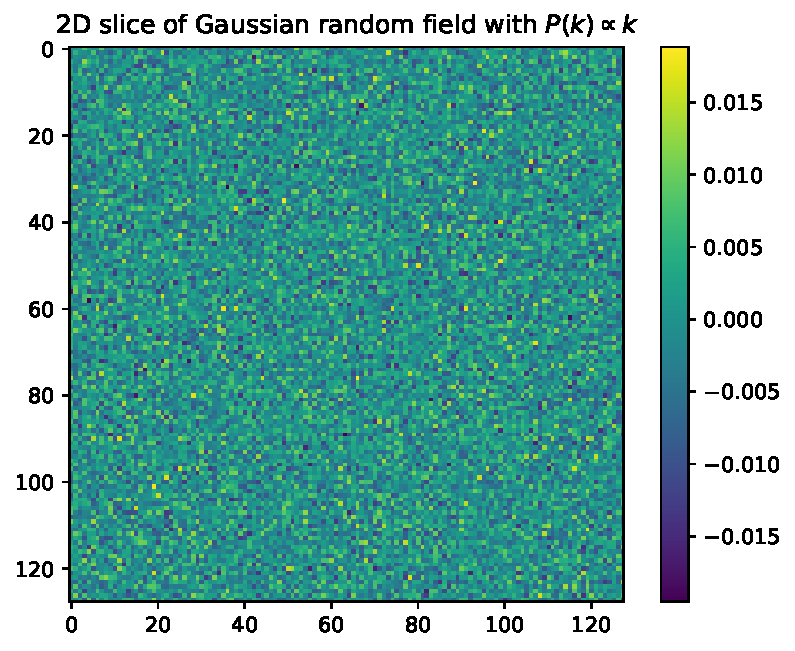
\includegraphics[width=0.7\linewidth]{../gaussian_random_field/GRF-scale-invariant-spectrum}
	\label{fig:grf-scale-invariant-spectrum}
\end{figure}

\pagebreak

\subsection{Matter power spectrum from linear theory}
Initial matter power spectrum generated by inflation is $P(k) \propto k$. The change in form of power spectrum in the linear regime is given by transfer function. We use BBKS fit for the transfer function and set Hubble constant to be $ 70$ (km/s)/Mpc, $h=0.7$.

\begin{figure}[H]
	\centering
	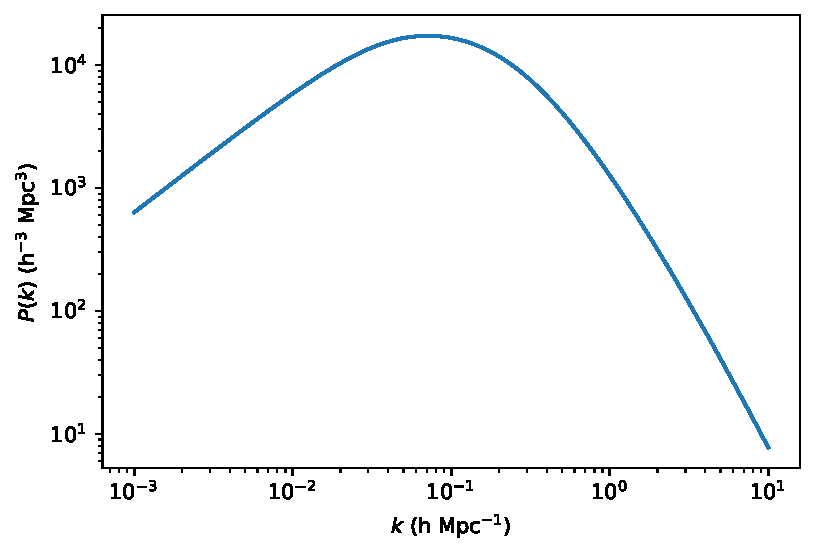
\includegraphics[width=0.7\linewidth]{../jupyter-nb/standard-cdm-matter-Pk}
	\caption{Matter power spectrum in CDM model ($\Omega_m=1$ \& $h = 0.7$)}
	\label{fig:standard-cdm-matter-pk}
\end{figure}
We can see that the power spectrum has different forms in the small scale and large scale limit. If we now include dark energy, then the transition happens at relatively large scale.

\begin{figure}[H]
	\centering
	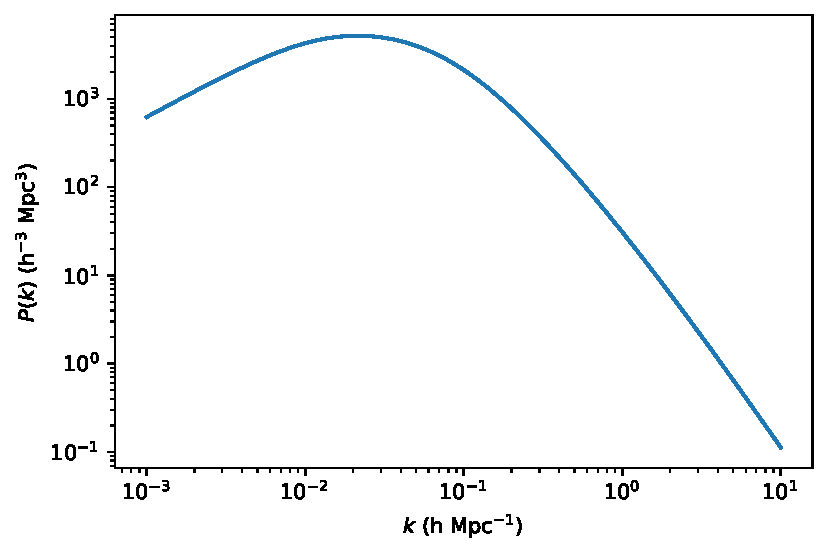
\includegraphics[width=0.7\linewidth]{../jupyter-nb/lambda-cdm-matter-Pk}
	\caption{Matter power spectrum in $\Lambda$-CDM model ($\Omega_m=0.3$ \& $h = 0.7$)}
	\label{fig:lambda-cdm-matter-pk}
\end{figure}
%width=0.7\linewidth

Inflation gave only the form of the initial power spectrum, we have to normalise bysing observational constraint.
\subsubsection*{$\sigma_8$ normalisation}
$\sigma_8$ is defined as the root mean square of density variation after smoothing by correlating with spherical top-hat function of radius 8 h$^{-1}$ Mpc. In the Fourier space, this is equivalent to multiplying by the Fourier transform of that top-hat function.
\begin{align}
W_s(k) &= 3 ~\frac{j_1(k R_8)}{k R_8} \quad \text{where } R_8 = 8 \text{ h$^{-1}$ Mpc}
\end{align}
Hence
\begin{align}
\sigma_8 &= \sqrt{ \frac{1}{(2 \pi)^3} \int W_s^2(k) ~|\delta (\vec{k})|^2 ~d^3k}\\
\sigma_8^2 &=  \frac{1}{(2 \pi)^3} \int W_s^2(k) ~|\delta (\vec{k})|^2 ~d^3k\\
&= \frac{1}{(2 \pi)^3} \int W_s^2(k) ~|\delta (\vec{k})|^2 ~k^2 dk ~d\Omega\\
&= \frac{1}{(2 \pi)^3} \int W_s^2(k) ~k^2 dk \int |\delta (\vec{k})|^2  ~d\Omega\\
&= \frac{1}{(2 \pi)^3} \int W_s^2(k) ~k^2 ~4\pi P(k) ~dk\\
&= \frac{1}{2 \pi^2} \int W_s^2(k) ~k^2 ~P(k) ~dk\\
&= \int W_s^2(k) ~\Delta^2(k) ~d(\ln k)
\end{align}
%
The integrand becomes negligible away from the Fourier mode of 8 h$^{-1}$ Mpc scale.\\
This quantity $\sigma_8$ is compared with the observations to fix the normalisation constant.

%\subsubsection*{Generating GRF from power spectrum}

\section{N-body simulations}
Numerically solving

%\subsection{Particle approach}
%
%\subsection{Grid approach}


\subsection{Snapshot of a GADGET-2 simulation}
\cite{aseem_shadab}

\begin{figure}[H]
	\centering
	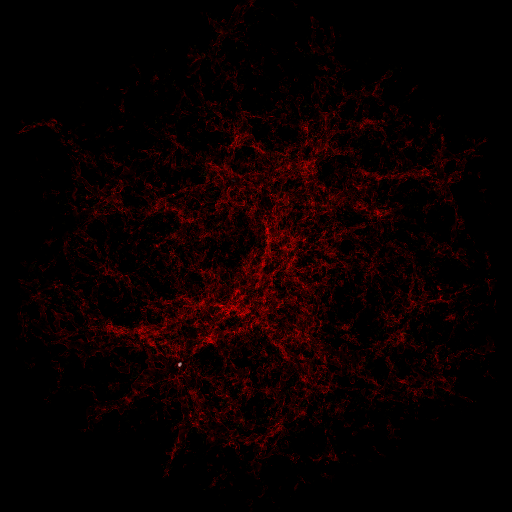
\includegraphics[width=0.5\linewidth]{../density_assign/UniformGridData_Render_density}
	\caption{Density field from the snapshot \quad
		 Volume rendered with yt-project}
	\label{fig:uniformgriddatarenderdensity}
\end{figure}


\section{Conclusion and Future plan}




\begin{thebibliography}{widest entry}
%\bibitem[GADGET]{cite_key1} bibliographic information
\bibitem[SDSS]{cite_sdss} \url{https://www.sdss.org/science/}
\bibitem[simulation]{aseem_shadab} Aseem Paranjape, Shadab Alam, Voronoi volume function: a new probe of cosmology and galaxy evolution, Monthly Notices of the Royal Astronomical Society, Volume 495, Issue 3, July 2020, Pages 3233–3251, \url{https://doi.org/10.1093/mnras/staa1379}
\end{thebibliography}






\end{document}